\chapter{Related Work}

%%% INTRO

In this chapter we briefly review the state of the art regarding the creation of
event models from social media data.
%

This chapter is organized as follows. 
%
First, we review common tasks related to events on social media. 
%
We then review different models or representations of events with respect to
specific tasks, which is directly related to the following chapters, covering
this work. 
%
Finally, we review the literature involving quantitative analysis of news
events, also called {\em quantitative history}.



\section{Common Tasks involving Events}

Most of the research in social media event analysis has been focused on the
creation of event models for specific tasks such as detection, tracking,
summarization and characterization of events in social media streams. 
%
Typically, event information is represented as bag of words, {\em tf-idf}
vectors~\cite{tfidf,Marcus:2011:TAV:1978942.1978975}, language
models~\cite{zellers2019neuralfakenews}, probability distributions over
text~\cite{o2010tweetmotif,Hong:2010:EST:1964858.1964870,zhao2011comparing,Mehrotra:2013:ILT:2484028.2484166},
or graph
representations~\cite{Setty:2018:ENE:3209978.3210136,Lee:2013:KSK:2487575.2487711,Lee:2014:CCS:2661829.2661859}.
%
Some other works exploit domain-specific features, such as the occurrence of
hashtags~\cite{Kamath:2013:SDO:2488388.2488447},
URLs~\cite{Alonso:2015:WCW:2740908.2745397},
locations~\cite{Abdelhaq:EvenTweet:2013}, or a mixture of
them~\cite{castillo2011information}.
%
Below we mention different approaches for event detection, summarization,
exploration, and applications to news media.
%


\subsection{Event Detection} 
%
The goal of event detection on social media is to identify coherent
time-constrained topics from the content that is continuously being published.
%
For instance, the majority of the methods for event detection on Twitter rely on
frequency analysis, semantic analysis, graph modeling, machine learning methods,
or a mixture of them.
%
For example, Sakaki et al.~\cite{Sakaki2010} develop a system for earthquake
detection using Twitter.
%
The authors design a classifier to detect if a tweet is talking about an
earthquake or not, using several features related to time, location, and
information diffusion between users.
%
Another example is the work of Poblete et al.~\cite{poblete2018robust}, which
detects changes in tweet volume to detect earthquakes.
%
TwitInfo~\cite{Marcus:2011:TAV:1978942.1978975} is a system to detect events on
Twitter, based on a set of features, such as content (bag of words and tf-idf
vectorization), sentiment values, and time (detecting peaks in tweet volume).
%
Semantic methods involve the study of the relationship between $n$-grams in the
text to detect topics or events, such as the work of Cai et
al.~\cite{cai2015popular}, which relies on topic models (such as Latent
Dirichlet Allocation) to detect events.
%
Graph modeling approaches attempt to extract a graph representation of messages
and then find appropriate sub-graphs that resemble events, such as the work of
Lee et al.~\cite{Lee:2013:KSK:2487575.2487711,Lee:2014:CCS:2661829.2661859}.
%
Machine learning methods, such as clustering and classification, are also used
to detect events.
%
Becker et al.~\cite{Becker:2010:LSM:1718487.1718524} proposed an incremental
clustering approach that groups messages if they are similar above a threshold.
%
This threshold is set empirically, but the features used for similarity are
fine-tuned for the application.
%
TwitterStand~\cite{Sankaranarayanan:2009:TNT:1653771.1653781} is a system
designed using similar principles as the previous work mentioned.
%
Certain studies focused specifically on the task of detecting events and tagging
their relevant geo-locations.  
%
In particular, some works targeted the detection of localized
events~\cite{Watanabe:Jasmine:2011,Abdelhaq:EvenTweet:2013,Walther:2013fb,Lee:A:2011,Krumm:2015},
others the detection of global events~\cite{sankaranarayanan:twitterstand:2009},
and the detection of critical
events~\cite{Sakaki:Tweet:2013,DeLongueville:2009}.
%
Dong et al.~\cite{Dong2015}, specifically, considered that events had different
temporal and spatial scales and proposed a multi-scale event detection approach
for social media.
%
This approach detects and reports events with geo-localization.
%
Another approach is to use information extraction techniques to identify named
entities, location names, etc. from Twitter
data~\cite{Ritter:2012:ODE:2339530.2339704}.
%
Temporal features for events have been used in tasks such as the detection of
events based on the temporal dynamics of their mentions in social
media~\cite{guille2015event}, and also for event
categorization~\cite{Ritter:2012:ODE:2339530.2339704}. 
%
The task in mind in this case is to perform event linking, that is, to match the
same news from different sources.
%
An extensive survey of event detection methods on Twitter can be found
in~\cite{hasan2018survey}.



\subsection{Automatic Summarization of Events} 
%
Event summarization methods aim to output a brief summary of an event.
%
These methods optimize certain criteria, such as relevance (the summary has to
be relevant to the event), diversity or coverage (the same aspects of the event
must be present in the summary), conciseness (not to have redundant information), 
and so on.
%
In this case, current methods attempt to select the most relevant pieces of
content in order to create a summary\footnote{This is known as {\em extractive
summarization}, as opposed to {\em abstractive summarization}, which creates its
own description of the event, not necessarily using content already in the
data.}, by identifying relevant aspects of the event and then selecting the most
important pieces of content.
%
Chakrabarti and Punera~\cite{chakrabarti2011event}, for example, used hidden
Markov models to represent sub-events within a broader event that is described
using Twitter data. 
%
This model identifies the corresponding time-intervals in which something
relevant happened, and then uses standard cosine similarity over the tf-idf
vectors to extract the most relevant tweets (see also Meladianos et
al.~\cite{meladianos2018optimization}).
%
Similarly, Alsaedi et al.~\cite{alsaedi2016temporal} proposed a way to process
large amounts of data by splitting the dataset into time-framed segments, and
then summarizing each frame using a tf-idf based approach.
%
Another approach was presented in a previous work of
ours~\cite{quezada2013understanding}, in which we focused on automatic
summarization of multimedia content by using social media posts as surrogate
text for multimedia documents.
%
In this case, we clustered similar groups of posts that shared the same URLs,
and then selected the most salient pieces of content from each cluster.
%
A similar approach was used by Alonso et
al.~\cite{Alonso:2015:WCW:2740908.2745397}, which was based on the \emph{social
signature} of documents (defined as the set of keywords of social media messages
that point to a document), to augment document metadata.
%
MGraph~\cite{schinas2016mgraph} was designed to detect topics on images and text
simultaneously from Twitter event data, extracting the most important posts
and images to create a summary.
%
The authors represented posts and images as a similarity graph and then ranked
the most relevant pieces of content.
%
Likewise, Xu and Lu~\cite{Xu:2015:SBP:2678025.2701385} represented Tumblr posts
as a graph and then ranked the posts in order to extract a summary.
%
Bian et al.~\cite{bian2014multimedia} represented events using graphical models
with textual and visual features of text and images from Sina Weibo,
respectively.
%
Similarly, the output of their model is the set of relevant images and texts,
which fulfill their criteria.

\subsection{Systems for Event Exploration}
%
Diverse event exploration systems have been proposed in the literature.
%
These systems refer to tools to gain insights about events using large-scale user-contributed data.
%
In the work of Kamath et al.~\cite{Kamath:2013:SDO:2488388.2488447}, the authors
analyzed Twitter \emph{hashtags} in a large-scale study of the spatio-temporal
dynamics of {\em memes}, or pieces of information, such as a post, an image, or
a video. 
%
In this work, a hashtag was represented as a tuple consisting of the coordinates
of the hashtag's location over time. 
%
They used a simple model to find interesting insights about the adoption and
spread of memes in social media. 
%
Memes are information units which emerge from social networks and can spread in
a viral way. 
%
However, meme dissemination does not necessarily resemble how other types of
information will propagate, such as information about events that originate
outside of the network (i.e., exogenous events), or that originate from
different sources at the same time.
%
Saravanou et al.~\cite{Saravanou:Twitter:2015} identified areas of interest
after floods in the UK using tweets, by clustering messages based on their
geographical coordinates and then selecting the most relevant messages from the
most dense areas.
%
Alonso et al.~\cite{Alonso:2017:WHH:3091478.3091484} designed a system for
exploring popular trends. 
%
The authors represented collections of tweets as diffusion trees, by
aggregating tweets by shared URLs and then computing popularity metrics of each
tree, and finally presenting the most relevant URLs with corresponding tweets.
%
Wang et al.~\cite{Wang:LeadLine:2012} visualized topics based on the extraction
of geographical entities from tweet text. 
%
They did not use this information to establish the location of an event, but
rather for event exploration.
%
SensePlace2~\cite{MacEachren:SensePlace2:2011} is a Visual Analytics tool that
allows users to explore a set of tweets and models them by showing two
geographical types of information: the locations from where users discussed the
topic and the locations being mentioned in tweets. 
%
However, this information was only used at single tweet level.


\subsection{Improving News Delivery from Social Media}
%
Related work has also approached the analysis of social media data in order to support or
improve news delivery. 
%
For example, \v{S}tajner et al.~\cite{Stajner:2013:ASS:2487575.2487659} proposed
an optimization problem to select the most interesting response to a news
article, where responses are tweets.
%
Diakopoulos et
al.~\cite{Diakopoulos:2012:FAS:2207676.2208409,diakopoulos2010diamonds} designed
a system to explore news events with journalists as the target users.
%
The authors propose different features they deemed relevant for their use
case: relevance, uniqueness, sentiment, verity, etc. 
%
The study of the spread of rumors, ``fake news'' and the veracity of content is
a very active field to the date of this dissertation.
%
The work of Castillo et al.~\cite{castillo2011information} is one of the first
approaches to this problem, where the authors investigate the characteristics of
rumors as they spread in Twitter, and developed a classifier using several
content, network, and user-based features.
%

From another point of view, {\em Culturomics} is defined as {\em the application
of high-throughput data collection and analysis to the study of human
culture}~\cite{Michel176}. 
%
The term was first introduced in a {\em Science} article from 2010, where the
authors studied the contents of about 5 million digitized
books~\cite{Michel176}. 
%
Our focus is on the development of information models in the context
of news events for studying trends and culture.
%
In the sense of information models, Suchanek and
Preda~\cite{Suchanek:2014:SC:2732977.2732994} proposed the term ``Semantic
Culturomics,'' or the use of knowledge bases and Semantic Web techniques to give
structure to human-generated data to obtain new insights.
Leetaru~\cite{leetaru2011culturomics} proposed the application of culturomics to
news events, applying standard Natural Language Processing techniques to
traditional media, finding insights about international relations.
%
GDELT~\cite{leetaru2013gdelt} is one example of the application of culturomics
to the traditional news media: it is a collection of news events with
automatically added metadata, such as locations, sentiment, entities, etc.


\section{Event Models}

In the context of social media, there are scattered attempts to create an
unified system to collect and annotate events, mainly due to the noisy nature of
user-contributed messages.
%
The presence of irrelevant, redundant, or untrustworthy messages make it
difficult to have robust models in social media.
%
Most of the representations proposed in the literature are tailored to specific
applications in Information Retrieval, specifically, in Topic Detection and
Tracking~\cite{allan2012topic} (TDT) tasks.
%
On social media, studies on news events have been used for diverse tasks,
such as event detection, tracking, prediction, sentiment analysis,
summarization, and virality. 
%

In this section, we review event models designed for specific tasks and
contexts. 
%
In particular, we review studies of representations of event impact, temporal
and location-aware context, and content aggregation for improving event
representation.


% Brief background on the problem
\subsection{Modeling the Impact of Events}

The study of information propagation on the Web has sparked tremendous interest
in recent years. 
%
Current literature on the subject primarily considers the process through which
a {\em meme}, usually a piece of media (like a video, an image, or a specific
Web article), gains popularity, and its popularity is measured through a certain
metric, such as the number of retweets, favorites or likes, and so
on~\cite{Castillo:2014,Szabo:2010,Lerman:2010,Tatar2014,Pinto:2013,Ahmed:2013,Li:2016:concept:drift,
Liu:2015:UN,10.1145/1963192.1963222,ICWSM112754}. 
%
However, a meme represents a simple information unit and its propagation
behavior does not necessarily correspond to that of more complex information
such as news events. 
%
News events are usually diffused in the network in many different formats, e.g.,
a particular news story such as an {\em earthquake in Japan} can be communicated
through images, URLs, tweets, videos, etc. 
%
Therefore, current research can benefit from analyzing the effects of more
high-level forms of information. 

\begin{figure}
    \centering
    \begin{subfigure}[b]{\textwidth}
        \centering 
        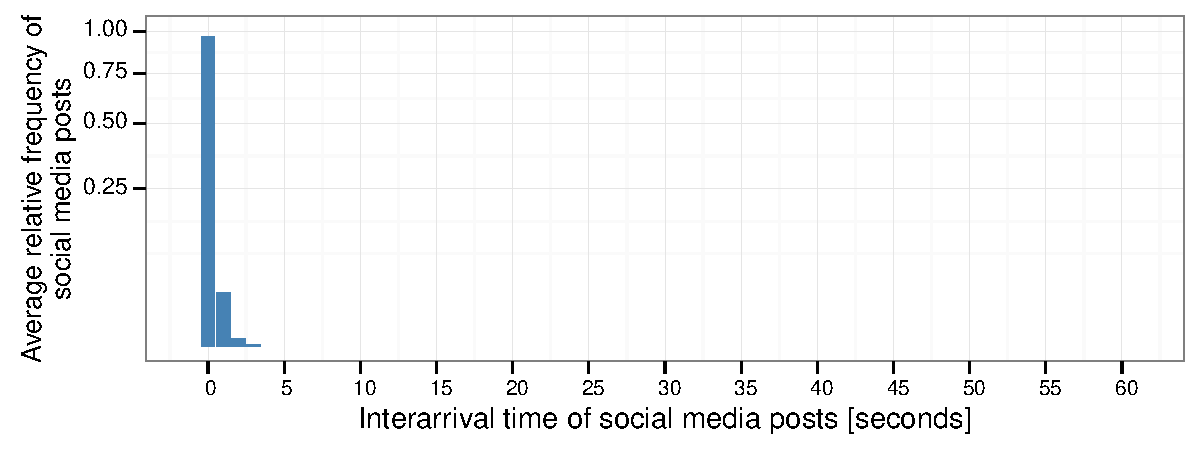
\includegraphics[width=.8\textwidth]{figures/high-activity/fig1a}
        \caption{Death of Nelson Mandela}
        \label{fig:hi:example-mandela}
    \end{subfigure}
    
    \begin{subfigure}[b]{\textwidth}
        \centering
        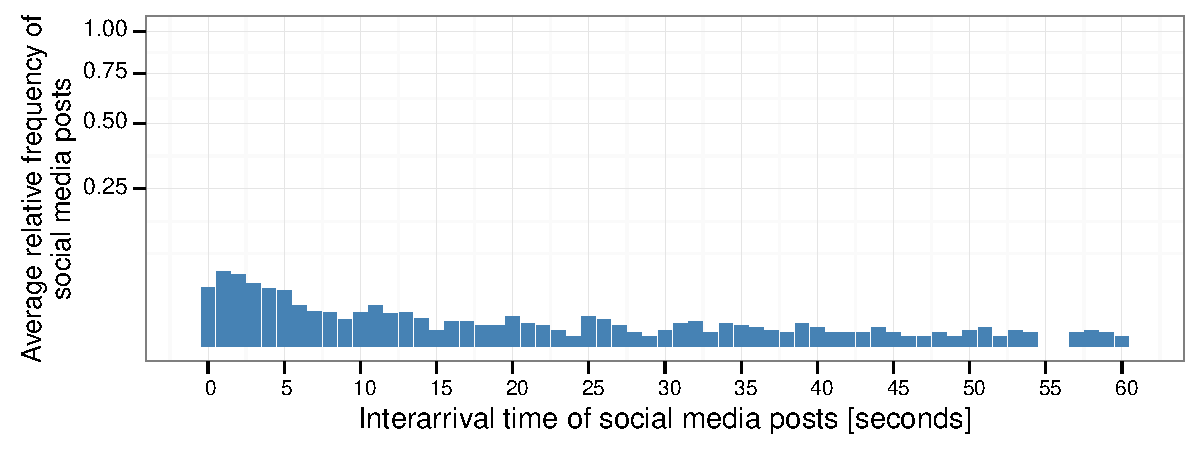
\includegraphics[width=.8\textwidth]{figures/high-activity/fig1b}
        \caption{One week after 2014 The Oscars}
        \label{fig:hi:example-oscars}
    \end{subfigure}

    \caption[Example histograms of time differences between tweets]{Histograms
        of the time differences between consecutive tweets in two example
        events: the death of Nelson Mandela (collected on 2013-12-05) and the
        commentary about the 2014 Oscars, several weeks after the main event
        (collected on 2014-03-23). Since there is a high concentration in the
        first histogram bin for the first histogram, we conclude that the social
        media posts for this event occur in cascades of quick successions,
        almost instantaneously. The arrival times of the posts on the second
        event are much more spread out. The $y$-axis is in square root scale.}
    \label{fig:hi:examples}
\end{figure}

Traditionally, the impact of information in online social networks has been
measured in relation to the total amount of attention that this subject receives
\cite{berger2012makes,iribarren2011branching,guerini2011exploring,mills2012virality,gaugaz2012predicting}.
%
That is, if a content posted in the network receives votes/comments/shares above
a certain threshold it is usually deemed as {\em viral} or {\em popular}.
%
Nevertheless, this notion of popularity or impact will favor only information
that produces very large volumes of social media messages. 
%
Naturally, global breaking news that has world-wide coverage and that produces a
high volume of activity in a short time should be considered as having a strong
impact on the network (Figure~\ref{fig:hi:example-mandela}).  
%
However, there are other types of events that can produce a similar reaction in
smaller online communities such as, for example, on users from a particular
country (e.g., the withdrawal of the main right wing presidential candidate in
Chile due to psychiatric problems, just before
elections~\cite{chile_elections}). 
%
Clearly, events of local scope do not produce as much social media activity as
events of global scope, but they can create a strong and immediate reaction from
users in local networks~\cite{ReisBOPKA15}. 
%
Conversely, there are large events which do not produce an intense reaction,
such as {\em The Oscars} (Figure~\ref{fig:hi:example-oscars}), which span a long
period of time and are discussed by social network users for weeks or even
months, but do not spark intense user activity. 
%
Therefore, it is reasonable to consider additional dimensions, rather than just volume,
when analyzing the impact of information in online communities.  

Prior research has shown that certain types of individual activities, such as
communications (studied in email exchanges), work patterns and entertainment,
follow a behavior of bursts of rapidly occurring actions followed by long
periods of inactivity~\cite{barabasi2005origin}, referred to as {temporally
in-homogeneous} behavior~\cite{karsai2012universal}.  
%
This type of behavior initially observed in individual activities, has also been
observed in relation to other naturally occurring types of collective phenomena
in human dynamics similar to processes seen in self-organized
criticality~\cite{karsai2012universal}.  
%
In particular, extremely high-activity bursty behavior seems to also occur in
critical situations, observed from the information flow in cell phone networks
during emergencies\cite{gao2014quantifying}.  
%
Although, there is research towards modeling this type of collective behavior
\cite{yan2013information} in online social networks, to the best of our
knowledge, it has not yet been analyzed quantitatively.


%%%% GEO


\subsection{Location-aware Event Models}\label{sec:geo-related}

Certain studies focused specifically on the task of detecting events and tagging
their relevant geo-locations. 
%
In particular, some works targeted the detection of localized
events~\cite{Watanabe:Jasmine:2011,Abdelhaq:EvenTweet:2013,Walther:2013fb,Lee:A:2011,Krumm:2015},
others the detection of global events~\cite{sankaranarayanan:twitterstand:2009},
and the detection of critical
events~\cite{Sakaki:Tweet:2013,DeLongueville:2009}.  
%
Dong et al.~\cite{Dong2015}, specifically, considered that events had different
temporal and spatial scales and proposed a multi-scale event detection approach
for social media. 
%
This approach focuses on detecting and reporting events with geo-localization.
%
Our current approach differs from existing work, in that we create an aggregated
representation of the information about real-world events, producing a
high-level representation that includes the event's geographical context, which
is extracted from social media. 
%
In addition, we enrich the information about an event by using the locations of
the users that post information about it.

Wang et al.~\cite{Wang:LeadLine:2012} visualized topics based on the extraction
of geographical entities from tweet text. 
%
They did not use this information to establish the location of an event, but
rather for event exploration. 
%
SensePlace2~\cite{MacEachren:SensePlace2:2011} is a Visual Analytics tool that
allows users to explore a set of tweets and models them by showing two
geographical types of information: the locations from where users discussed the
topic and the locations being mentioned in tweets. 
%
However, unlike our work, this information was only used at the single tweet level,
and not at event level.

In the domain of cyber-physical systems, {\em events} are viewed as conditions
of interest~\cite{st-model_2009} within a cyber-physical system, or as the
co-occurrence of two people in the same physical place~\cite{STEvent_2010}.
%
In general, events are modeled according to the state of the objects in the
system, considering attributes, time and location. 
%
The work presented by Tan et al.~\cite{st-model_2009} bears certain similarities
with our own, in the sense that they considered an event to encompass multiple pieces of 
information about a condition of interest in the system (in our case in the
online social network), including time and physical locations. 
%
In addition, the authors defined different kinds of temporal and geographical
scopes for their events, which are similar to our definition of {\em event
impact}. 
%
The main difference is that our approach aims to capture high-level
information of how a complex exogenous event, such as a news event, is perceived
by social network users in an aggregated way. 
%
Therefore, we focus on geopolitical divisions as units of aggregated spatial
information and on representing geopolitical interactions.

%%

Although the idea of adding spatio-temporal context to social media data is
not novel, to the best of our knowledge our work is the first that formally
introduces {\em protagonist} and {\em interested} locations in a high-level
event representation.  
%
The novelty of our approach relies on the extension of the notion of spatial
context, first by associating real-world news to one or more protagonist
locations, and second by associating real-world news to the locations where they
generated interest.  
%
In addition, our work does not focus on event detection, classification or
summarization, as most of the prior work on event analysis does.




%%%%% URL models
\subsection{Models of Aggregated Event Content}\label{sec:url-related}
% There is extensive work on automatic summarization on microblogs\mq{ref}. In
% this work, we approach the problem from a practical point of view, where our
% goal is to benefit from the characteristics of social media posts, in
% particular, from event-related messages. We exploit the redundancy of
% information available in social media via the aggregation of information
% around shared URLs, and propose a simple and compact model using word
% embeddings on tweets. Therefore, we can classify the related work in three
% areas: modeling social media content, automatic summarization of news, and
% usage of word embeddings in social media.


The use of anchor texts to represent content comes from the
development of the first search engines, in which content was represented by the
queries that users made to find the documents containing that
content~\cite{10.1145/345508.345597,ilprints422,amitay1998using}.
%
In this work we are interested in the use of anchor texts in the context of
microblogs.
%
Two lines of research are relevant to our work: the utility of anchor
texts and topic detection methods using different aggregation
strategies. 
%
In this section, we briefly review related work in those two lines.

%
Raux et
al.~\cite{raux2011describing} used anchor texts from tweets pointing to a
predefined set of URLs to characterize general topics, by clustering a bipartite
graph of words and URLs. 
%
We instead focus on news events, and tweets related to these news, which have
their own particularities, in contrast to long lasting general topics. 
%
Mishne and Lin~\cite{mishne2012twanchor} studied the contribution of anchor
texts compared to the text of the websites behind the URLs, concluding that
anchor text add new terms not seen in the website content, by looking also at
the conversations around the sharing tweets. 
%
Alonso et al.~\cite{Alonso:2015:WCW:2740908.2745397} had similar findings
examining Facebook posts. 
%
In another work by Alonso et al.~\cite{Alonso:2017:WHH:3091478.3091484}, the
authors designed a social search engine using the propagation of shared URLs as
cues to measure virality, and anchor texts to augment metadata of the search
results with social content. 
%
In a previous work~\cite{quezada2013understanding}, we showed a proof of concept
of automatic summarization of documents using anchor texts.
%


Topic modeling of tweets is an active line of research, and there are some
studies which investigate the effectiveness of aggregation of tweets to improve
topic
detection~\cite{Hong:2010:EST:1964858.1964870,Mehrotra:2013:ILT:2484028.2484166,alvarez2016topic}.
Hong and Davison~\cite{Hong:2010:EST:1964858.1964870} analyzed the effects of
different aggregation strategies of tweets when finding topics with Latent
Dirichlet Allocation (LDA). 
%
They found that some schemes yield better results at some tasks, such as
classification problems related to tweets. 
%
In a similar fashion, Mehrotra et al.~\cite{Mehrotra:2013:ILT:2484028.2484166}
observed that aggregating hashtags (also described as {\em pooling} of tweets by
hashtags) is a more effective strategy to identify topics from tweets, but at
the cost of longer running times due to the duplication of tweets. 
%
Finally, Alvarez-Melis and Saveski~\cite{alvarez2016topic} found that adding the
threads of conversation into the pooling is more effective than pooling by
hashtag in their observations. 
%
We instead aggregate by shared URLs and conversations, with the goal of
generating a compact representation without major loss of information.



% \subsection{Using common information in tweets}

% Similar to our work, in the sense of exploiting common information across
% messages, the work of Kamath et al.~\cite{Kamath:2013:SDO:2488388.2488447}
% focuses in the spatio-temporal dynamics of {\em memes}, as seen as units of
% information spreaded in social media. For this, they model each tweet as a
% tuple of the hashtags involved, time, and location to observe and characterize
% topics in Twitter. Similarly, the work of Pe\~na-Araya et
% al.~\cite{pena2017gaining} aim to characterize geopolitical entities (such as
% countries) based on the tweets that mention them, by proposing a model to
% represent locations in a spatio-temporal ambit, and develop a visual analytics
% tool to explore events based on the location scope of their impact. Our work
% is similar to both in the sense of leveraging common entities across messages,
% in this case, the URLs, in order to generate a compact representation to
% facilitate the discovering of sub-events. In our case, we do so by using URLs
% and the text content as a surrogate for the URLs, also called anchor texts.

% Concerning the specific use of anchor text in social media, Mishne and
% Lin~\cite{mishne2012twanchor} show that the anchor texts in general tweets
% provide additional new information compared to the content of webpages alone
% in a study of 7 million URLs obtained from the Twitter Firehose. The work of
% Raux et al.~\cite{raux2011describing} is one of the first to use anchor texts
% to find clusters of topics in Twitter, in order to describe Web content using
% tweets. The authors create a weighted bipartite graph of tweet words and URLs,
% being the weight the tf-idf score of the words in the tweets that contain the
% URL, and then find clusters of URLs. Although they characterize clusters of
% URLs as topics, their work focuses on general tweets and not newsworthy
% messages in particular. In the work of Alonso et
% al.~\cite{Alonso:2017:WHH:3091478.3091484}, the authors develop a search
% engine for content related to URLs shared on Twitter, displaying the most
% popular and viral URLs, also showing the effectiveness of this approach. In
% our previous work~\cite{quezada2013understanding}, we show a prototype of a
% automatic summarization methodology using tweets aggregated by URL, and then
% modeling the aggregated sets as tf-idf vectors to cluster them, find sub-events, 
% and then selecting the most representative messages as a multi-modal
% summary.




% \subsection{Applications of tweet representations}

% Automatic text summarization has been employed in different domains, such as
% news~\mq{cite}, sports~\cite{meladianos2018optimization,chakrabarti2011event},
% music~\cite{raposo2016using}, or movies~\cite{aparicio2016summarization}.

% There are several approaches for automatic summarization of events from social
% media, being many of them inspired in automatic text summarization. In order
% to manage scale, most of the related approaches do not deal with all the data
% at once, but work with similar sub-problems, such as sub-events detected via
% time windows, clustering, or online approaches. 

% The work of Chakrabarti and Punera~\cite{chakrabarti2011event} identifies
% particular time windows in structure-rich events, such as football matches.
% Using Hidden Markov Models, the authors find time windows associated with
% specific sub-events (e.g., a "touchdown") and then summarize each sub-event
% using a centroid-based approach on the tf-idf representation of the tweets.
% Similarly, Alsaedi et al.~\cite{alsaedi2016temporal} fix a time window of one
% hour to define all the tweets in that time window as a cluster, and then use
% two consecutive clusters to take into account the changes between time
% windows. They also propose two additional approaches, namely using a retweet
% voting approach and a temporal centroid method. In all cases, the approaches
% do not use all the dataset at once, but select a limited amount of messages as
% a sub-event. 

% We do not follow this approach, mainly because different sub-events  
% may be mentioned in different stages of the event, and the time-window
% approach can result in low purity clusters when being applied to general
% events.


% One of the first online approaches to event detection and summarization in
% Twitter is the work of Sankaranarayanan et
% al.~\cite{Sankaranarayanan:2009:TNT:1653771.1653781}. The authors describe a
% system that collects tweets and identifies events using an online clustering
% procedure over a tf-idf representation of tweets. \mq{problema con esto}



\section{Quantitative Analysis of News Events}

We provide a review of the literature on {\em quantitative history} research
applied to event analysis and social media. 
%
Quantitative history is an approach to historical research that makes use of
quantitative and digital tools. 


Prior work used digitized newspapers and books for extracting quantitative
knowledge~\cite{Michel176,leetaru2011culturomics,chadefaux2014early}. 
%
Michel et al.~\cite{Michel176} built a corpus of 5 million books and analyzed
them using word frequencies to investigate cultural trends, and called this type
of study ``Culturomics.''
%
Chadefaux~\cite{chadefaux2014early} used a dataset from Google News Archive to
predict military conflicts.
%
Leetaru~\cite{leetaru2011culturomics} performed a large-scale study of 30 years
of digitized newspapers.
%
The author computed sentiment scores and geo-location for each article.
%
The study suggested that some critical events in the past, such as social
revolutions, could have been forecast by looking at sentiment scores over
time.
%
In addition, the author performed community detection on country graphs by
analyzing news in which two or more countries were involved.  
%
In this sense, our approach is similar, because we model locations in terms of
their co-occurrence in news. 
%
However, our work is focused on automatic information extraction from online
social streams and on the creation of a more general representation.  
%
We do not focus on the analysis of sentiment of edited content from formal news
media outlets, but on the interactions between locations, based on the
aggregated reactions and opinions of users of social platforms.
%


A different line of research covers digitized writings and the Semantic Web.
%
Suchanek and Preda~\cite{Suchanek:2014:SC:2732977.2732994} proposed the study of
``Semantic Culturomics'', in which the analysis of newspapers should go beyond
the study of word frequencies in order to integrate knowledge bases (such as
DBPedia~\cite{dbpedia}) to answer complex user queries. 
%
Additional research has used knowledge bases along with human writings, such as
newspapers~\cite{Huet:2013:MHL:2509558.2509567,DS/CN175}. 
%
A survey on this topic is provided by Mero\~no-Pe\~nuela et
al.~\cite{merono2014semantic}.

Castillo et al.~\cite{Castillo:2014} studied the traffic
that online news sources receive in response to news, finding two types of news
articles, based on their ``shelf-life'' in social media responses. 
%
Their findings are similar to ours when analyzing the characteristics of
high-activity events in Chapter~\ref{chapter:high-activity}.
%

The work of Setty and Hose~\cite{Setty:2018:ENE:3209978.3210136} aims to create
a common representation of events based on neural embeddings, using a procedure
similar to Node2Vec~\cite{Grover:2016:NSF:2939672.2939754}.
%
A general representation of events is useful to perform high-level quantitative
analysis, as it is flexible enough for arbitrary events.
%
However, it suffers from a lack of interpretability, as it is very difficult to determine
the underlying factors that produced a certain representation.
%
Sellam and Alonso~\cite{10.1007/978-3-319-19890-3_17} designed a system for
information extraction from news events on Twitter that extracts quantitative
data from events, such as dates, numbers, entities, etc.


Compared to prior work, our approach is among the first to consider user-generated
information networks, such as online social networks, which are a growing data
source at much larger scale.  
%
We consider that social media can provide additional and novel information to
that found in news articles and books. 
%
User-generated content reflects social opinions and points of view related to
current world-events. 
%
This content is generated in real-time, it is not edited and does not depend on
the editorial lines of formal news outlets.  
%
We believe that these unique characteristics make social media a challenging and
valuable source of historical information.  
%
Our approach incorporates the content of social media platforms about real-world
news, as well as aggregated geographical information that conveys the importance
and scope of these events.

%
